\documentclass{standalone}
\usepackage{tikz}
\usetikzlibrary{patterns, positioning}


\begin{document}
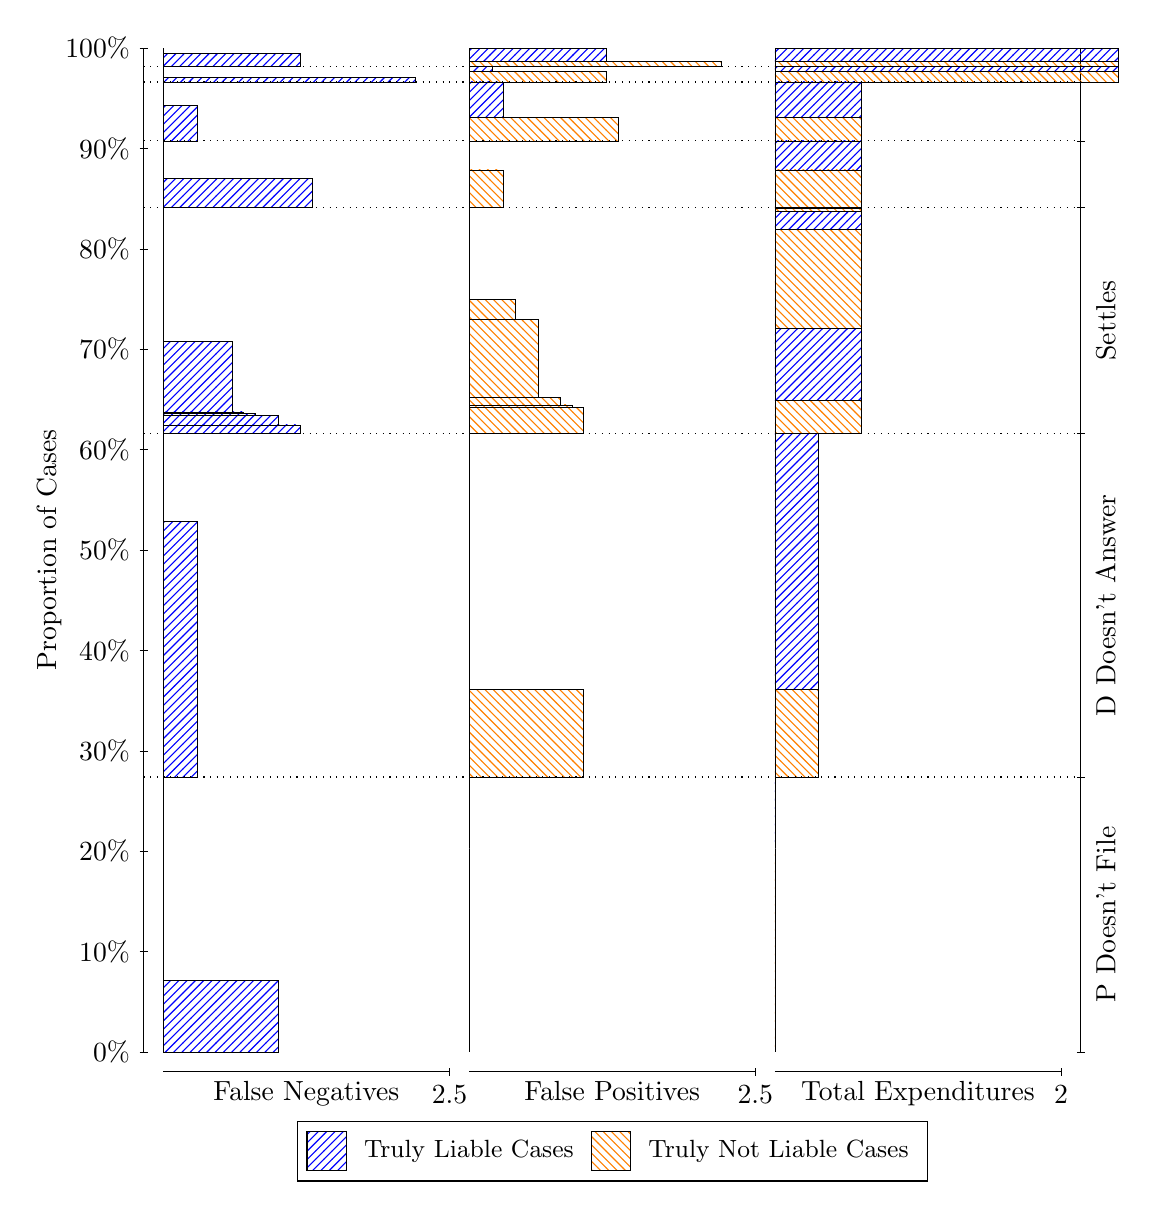
\begin{tikzpicture}
\draw[black, very thin] (1.5,1.75) -- (1.5,14.5);
\node[rotate=90, text=black, anchor=center] at (0.3, 8.125) {Proportion of Cases};
\draw[black, very thin] (1.45,1.75) -- (1.55,1.75);
\node[text=black, anchor=east] at (1.45, 1.75) {0\%};
\draw[black, very thin] (1.45,3.025) -- (1.55,3.025);
\node[text=black, anchor=east] at (1.45, 3.025) {10\%};
\draw[black, very thin] (1.45,4.3) -- (1.55,4.3);
\node[text=black, anchor=east] at (1.45, 4.3) {20\%};
\draw[black, very thin] (1.45,5.575) -- (1.55,5.575);
\node[text=black, anchor=east] at (1.45, 5.575) {30\%};
\draw[black, very thin] (1.45,6.85) -- (1.55,6.85);
\node[text=black, anchor=east] at (1.45, 6.85) {40\%};
\draw[black, very thin] (1.45,8.125) -- (1.55,8.125);
\node[text=black, anchor=east] at (1.45, 8.125) {50\%};
\draw[black, very thin] (1.45,9.4) -- (1.55,9.4);
\node[text=black, anchor=east] at (1.45, 9.4) {60\%};
\draw[black, very thin] (1.45,10.675) -- (1.55,10.675);
\node[text=black, anchor=east] at (1.45, 10.675) {70\%};
\draw[black, very thin] (1.45,11.95) -- (1.55,11.95);
\node[text=black, anchor=east] at (1.45, 11.95) {80\%};
\draw[black, very thin] (1.45,13.225) -- (1.55,13.225);
\node[text=black, anchor=east] at (1.45, 13.225) {90\%};
\draw[black, very thin] (1.45,14.5) -- (1.55,14.5);
\node[text=black, anchor=east] at (1.45, 14.5) {100\%};

\draw[black, very thin] (13.4,1.75) -- (13.4,14.5);
\draw[black, very thin] (13.35,1.75) -- (13.45,1.75);
\node[anchor=west] at (13.35, 1.75) {};
\draw[black, very thin] (13.35,5.242) -- (13.45,5.242);
\node[anchor=west] at (13.35, 5.242) {};
\draw[black, very thin] (13.35,9.606) -- (13.45,9.606);
\node[anchor=west] at (13.35, 9.606) {};
\draw[black, very thin] (13.35,12.478) -- (13.45,12.478);
\node[anchor=west] at (13.35, 12.478) {};
\draw[black, very thin] (13.35,13.32) -- (13.45,13.32);
\node[anchor=west] at (13.35, 13.32) {};
\draw[black, very thin] (13.35,14.069) -- (13.45,14.069);
\node[anchor=west] at (13.35, 14.069) {};
\draw[black, very thin] (13.35,14.269) -- (13.45,14.269);
\node[anchor=west] at (13.35, 14.269) {};
\draw[black, very thin] (13.35,14.5) -- (13.45,14.5);
\node[anchor=west] at (13.35, 14.5) {};

\draw[black, very thin, pattern color=blue, pattern=north east lines] (1.75,1.75) rectangle (3.2033,2.6608);
\draw[black, very thin, pattern color=orange, pattern=north west lines] (1.75,2.6608) rectangle (1.75,5.242);
\draw[black, very thin, pattern color=blue, pattern=north east lines] (1.75,5.242) rectangle (2.186,8.4894);
\draw[black, very thin, pattern color=orange, pattern=north west lines] (1.75,8.4894) rectangle (1.75,9.606);
\draw[black, very thin, pattern color=blue, pattern=north east lines] (1.75,9.606) rectangle (3.494,9.7137);
\draw[black, very thin, pattern color=blue, pattern=north east lines] (1.75,9.7137) rectangle (3.2033,9.8385);
\draw[black, very thin, pattern color=blue, pattern=north east lines] (1.75,9.8385) rectangle (2.9127,9.8608);
\draw[black, very thin, pattern color=blue, pattern=north east lines] (1.75,9.8608) rectangle (2.7673,9.8795);
\draw[black, very thin, pattern color=blue, pattern=north east lines] (1.75,9.8795) rectangle (2.622,10.772);
\draw[black, very thin, pattern color=orange, pattern=north west lines] (1.75,10.772) rectangle (1.75,12.478);
\draw[black, very thin, pattern color=blue, pattern=north east lines] (1.75,12.478) rectangle (3.6393,12.844);
\draw[black, very thin, pattern color=orange, pattern=north west lines] (1.75,12.844) rectangle (1.75,13.32);
\draw[black, very thin, pattern color=blue, pattern=north east lines] (1.75,13.32) rectangle (2.186,13.773);
\draw[black, very thin, pattern color=orange, pattern=north west lines] (1.75,13.773) rectangle (1.75,14.069);
\draw[black, very thin, pattern color=blue, pattern=north east lines] (1.75,14.069) rectangle (4.9473,14.132);
\draw[black, very thin, pattern color=orange, pattern=north west lines] (1.75,14.132) rectangle (1.75,14.269);
\draw[black, very thin, pattern color=blue, pattern=north east lines] (1.75,14.269) rectangle (3.494,14.436);
\draw[black, very thin, pattern color=orange, pattern=north west lines] (1.75,14.436) rectangle (1.75,14.5);
\draw[black, very thin, pattern color=orange, pattern=north west lines] (5.6333,1.75) rectangle (5.6333,4.3311);
\draw[black, very thin, pattern color=blue, pattern=north east lines] (5.6333,4.3311) rectangle (5.6333,5.242);
\draw[black, very thin, pattern color=orange, pattern=north west lines] (5.6333,5.242) rectangle (7.0867,6.3586);
\draw[black, very thin, pattern color=blue, pattern=north east lines] (5.6333,6.3586) rectangle (5.6333,9.606);
\draw[black, very thin, pattern color=orange, pattern=north west lines] (5.6333,9.606) rectangle (7.0867,9.9332);
\draw[black, very thin, pattern color=orange, pattern=north west lines] (5.6333,9.9332) rectangle (6.9413,9.9668);
\draw[black, very thin, pattern color=orange, pattern=north west lines] (5.6333,9.9668) rectangle (6.796,10.06);
\draw[black, very thin, pattern color=orange, pattern=north west lines] (5.6333,10.06) rectangle (6.5053,11.053);
\draw[black, very thin, pattern color=orange, pattern=north west lines] (5.6333,11.053) rectangle (6.2147,11.311);
\draw[black, very thin, pattern color=blue, pattern=north east lines] (5.6333,11.311) rectangle (5.6333,12.478);
\draw[black, very thin, pattern color=orange, pattern=north west lines] (5.6333,12.478) rectangle (6.0693,12.953);
\draw[black, very thin, pattern color=blue, pattern=north east lines] (5.6333,12.953) rectangle (5.6333,13.32);
\draw[black, very thin, pattern color=orange, pattern=north west lines] (5.6333,13.32) rectangle (7.5227,13.615);
\draw[black, very thin, pattern color=blue, pattern=north east lines] (5.6333,13.615) rectangle (6.0693,14.069);
\draw[black, very thin, pattern color=orange, pattern=north west lines] (5.6333,14.069) rectangle (7.3773,14.206);
\draw[black, very thin, pattern color=blue, pattern=north east lines] (5.6333,14.206) rectangle (5.924,14.269);
\draw[black, very thin, pattern color=orange, pattern=north west lines] (5.6333,14.269) rectangle (8.8307,14.333);
\draw[black, very thin, pattern color=blue, pattern=north east lines] (5.6333,14.333) rectangle (7.3773,14.5);
\draw[black, very thin, pattern color=orange, pattern=north west lines] (9.5167,1.75) rectangle (9.5167,4.3311);
\draw[black, very thin, pattern color=blue, pattern=north east lines] (9.5167,4.3311) rectangle (9.5167,5.242);
\draw[black, very thin, pattern color=orange, pattern=north west lines] (9.5167,5.242) rectangle (10.062,6.3586);
\draw[black, very thin, pattern color=blue, pattern=north east lines] (9.5167,6.3586) rectangle (10.062,9.606);
\draw[black, very thin, pattern color=orange, pattern=north west lines] (9.5167,9.606) rectangle (10.607,10.026);
\draw[black, very thin, pattern color=blue, pattern=north east lines] (9.5167,10.026) rectangle (10.607,10.941);
\draw[black, very thin, pattern color=orange, pattern=north west lines] (9.5167,10.941) rectangle (10.607,12.193);
\draw[black, very thin, pattern color=blue, pattern=north east lines] (9.5167,12.193) rectangle (10.607,12.425);
\draw[black, very thin, pattern color=orange, pattern=north west lines] (9.5167,12.425) rectangle (10.607,12.459);
\draw[black, very thin, pattern color=blue, pattern=north east lines] (9.5167,12.459) rectangle (10.607,12.478);
\draw[black, very thin, pattern color=orange, pattern=north west lines] (9.5167,12.478) rectangle (10.607,12.953);
\draw[black, very thin, pattern color=blue, pattern=north east lines] (9.5167,12.953) rectangle (10.607,13.32);
\draw[black, very thin, pattern color=orange, pattern=north west lines] (9.5167,13.32) rectangle (10.607,13.615);
\draw[black, very thin, pattern color=blue, pattern=north east lines] (9.5167,13.615) rectangle (10.607,14.069);
\draw[black, very thin, pattern color=orange, pattern=north west lines] (9.5167,14.069) rectangle (13.877,14.206);
\draw[black, very thin, pattern color=blue, pattern=north east lines] (9.5167,14.206) rectangle (13.877,14.269);
\draw[black, very thin, pattern color=orange, pattern=north west lines] (9.5167,14.269) rectangle (13.877,14.333);
\draw[black, very thin, pattern color=blue, pattern=north east lines] (9.5167,14.333) rectangle (13.877,14.5);
\draw[black, dotted] (1.5,5.242) -- (13.4,5.242);
\draw[black, dotted] (1.5,9.606) -- (13.4,9.606);
\draw[black, dotted] (1.5,12.478) -- (13.4,12.478);
\draw[black, dotted] (1.5,13.32) -- (13.4,13.32);
\draw[black, dotted] (1.5,14.069) -- (13.4,14.069);
\draw[black, dotted] (1.5,14.269) -- (13.4,14.269);
\draw[black, very thin] (1.75,1.5) -- (5.3833,1.5);
\node[text=black, anchor=north] at (3.5667, 1.5) {False Negatives};
\draw[black, very thin] (5.3833,1.45) -- (5.3833,1.55);
\node[text=black, anchor=north] at (5.3833, 1.45) {2.5};

\draw[black, very thin] (5.6333,1.5) -- (9.2667,1.5);
\node[text=black, anchor=north] at (7.45, 1.5) {False Positives};
\draw[black, very thin] (9.2667,1.45) -- (9.2667,1.55);
\node[text=black, anchor=north] at (9.2667, 1.45) {2.5};

\draw[black, very thin] (9.5167,1.5) -- (13.15,1.5);
\node[text=black, anchor=north] at (11.333, 1.5) {Total Expenditures};
\draw[black, very thin] (13.15,1.45) -- (13.15,1.55);
\node[text=black, anchor=north] at (13.15, 1.45) {2};

\node[text=black, centered, rotate=90] at (13.72, 3.496) {P Doesn't File};
\node[text=black, centered, rotate=90] at (13.72, 7.424) {D Doesn't Answer};
\node[text=black, centered, rotate=90] at (13.72, 11.042) {Settles};





\draw (7.449999999999999,1.5) node[draw=none] (baseCoordinate) {};
\begin{scope}[align=center]
        \matrix[scale=0.5, draw=black, below=0.5cm of baseCoordinate, nodes={draw}, column sep=0.1cm]{
            \node[rectangle, draw, minimum width=0.5cm, minimum height=0.5cm, pattern color=blue, pattern=north east lines] {}; &
            \node[draw=none, font=\small, text=black] (B) {Truly Liable Cases}; &
            \node[rectangle, draw, minimum width=0.5cm, minimum height=0.5cm, pattern color=orange, pattern=north west lines] {}; &
            \node[draw=none, font=\small, text=black] (B) {Truly Not Liable Cases}; \\
            };
\end{scope}

\end{tikzpicture}
\end{document}